\documentclass[main.tex]{subfiles}


\begin{document}


\section{Results}
\label{results}


\subsection{Strategy of SEARCH-MaP and SEISMIC-RNA}

% In Figure 1, the RNA sequence is CAAUGUGCCAAAGGUCAU (18 nt).
% This sequence could fold into the structures
% ..(((..((...)).))) [P--R interaction formed] and
% ((...))((...)).... [P--R interaction unformed].
% Since its purpose is only to illustrate a toy example, this sequence is never specified in the paper.

\begin{figure}[H]
	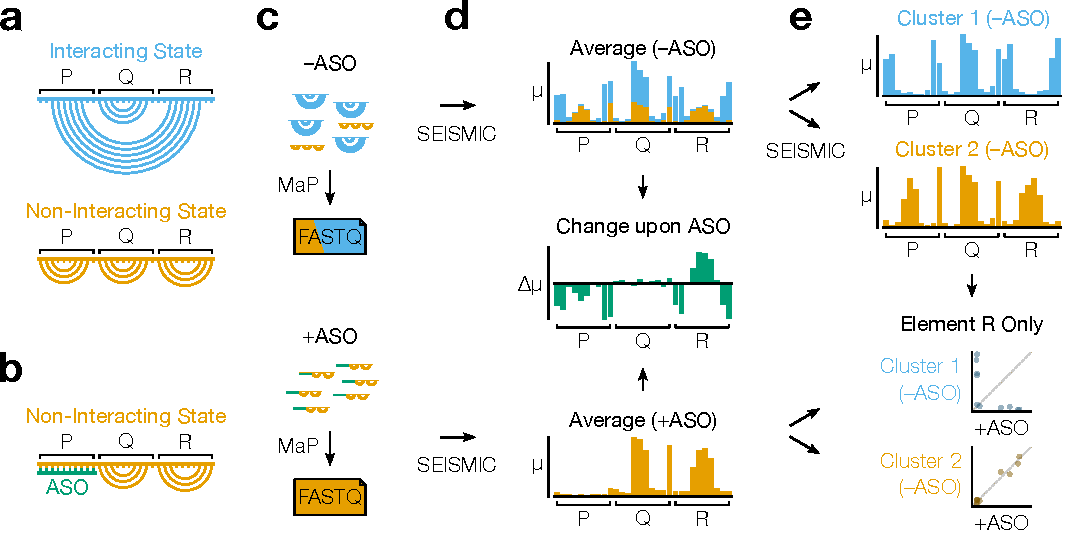
\includegraphics[width=\textwidth]{../MainFigures/strat.pdf}
	\caption{\textbf{The strategy of SEARCH-MaP and SEISMIC-RNA.} \textbf{(a)}~This toy RNA is partitioned into three sections (P, Q, and R) whose molecules exist in two structural states: one in which an interaction between P and R forms (blue) and one in which it does not (purple). \textbf{(b)}~Hybridizing an ASO (red) to P blocks it from interacting with R and forces all RNA molecules into the state where the P--R interaction is unformed. \textbf{(c)} A SEARCH-MaP experiment entails separate chemical probing and mutational profiling (MaP) with (+ASO) and without (--ASO) the ASO, followed by sequencing to generate FASTQ files. The RNA molecules and FASTQ files use the same color scheme as in (a) and are illustrated/colored in proportion to their abundances in the ensemble. \textbf{(d)} Ensemble average mutational profiles with (+ASO) and without (--ASO) the ASO, computed with SEISMIC-RNA. The \textit{x}-axis is the position in the RNA sequence; the \textit{y}-axis is the fraction of mutations ($\mu$) at the position. Each bar in the --ASO profile is drawn in two colors merely to illustrate how much each structural state contributes to each position; in a real experiment, states cannot be distinguished before clustering. The change upon ASO binding (green) indicates the difference in the fraction of mutations ($\Delta \mu$) between the +ASO and --ASO conditions. \textbf{(e)} Mutational profiles of two clusters (top) obtained by clustering the --ASO ensemble in (d) using SEISMIC-RNA, and the scatter plot of the mutation rates of bases in R (bottom) between the +ASO ensemble average (\textit{x}-axis) and each cluster (\textit{y}-axis). The expected correlation ($r$) is shown beside each scatter plot.}
	\label{strat}
\end{figure}

We illustrate SEARCH-MaP with an RNA comprising three sections (P, Q, and R) that folds into an ensemble of two structural states: one in which a base-pairing interaction between P and R forms, another in which it does not (Figure~\ref{strat}a).
Searching for sections that interact with P begins with hybridizing an antisense oligonucleotide (ASO) to P, which blocks P from base pairing with any other section, ablating the state in which the P--R interaction forms (Figure~\ref{strat}b).
The RNA is chemically probed separately with (+ASO) and without (--ASO) the ASO, followed by mutational profiling and sequencing, e.g. using DMS-MaPseq~\cite{Zubradt2016} (Figure~\ref{strat}c).

SEISMIC-RNA can detect RNA--RNA interactions by comparing the +ASO and --ASO mutational profiles.
Theoretically, each structural state has its own mutational profile~\cite{Sherpa2015}, but the mutational profile of a single state is not directly observable because all states are physically mixed during the experiment (Figure~\ref{strat}c, top).
Instead, the directly observable mutational profile is the ``ensemble average" -- the average of the states' (unobserved) mutational profiles, weighted by the states' (unobserved) proportions (Figure~\ref{strat}d, top).
Because the structures -- and therefore mutational profiles -- of R differ between the interaction-formed and -unformed states, the ensemble averages of R also differ between the +ASO and --ASO conditions (Figure~\ref{strat}d, middle).
However, this is not the case for element Q, which has the same secondary structure in both states (Figure~\ref{strat}d, middle).
Therefore, one can deduce that P interacts with R -- but not with Q -- because hybridizing an ASO to P alters the mutational profile of R but not of Q.

After identifying RNA--RNA interactions, SEISMIC-RNA can also determine the mutational profiles of the states where the P--R interaction is formed and unformed -- even if their secondary structures are unknown.
Inferring mutational profiles for the interaction-formed and -unformed states requires clustering the --ASO ensemble into two clusters of RNA molecules (Figure~\ref{strat}e, top).
Each cluster has its own mutational profile and corresponds to one structural state, but which cluster corresponds to the interaction-formed (or -unformed) state is not yet known.
The interaction-unformed state has a mutational profile similar to that of the +ASO ensemble average, since the ASO blocks the interaction and forces the RNA into the interaction-unformed state.
Therefore, a cluster that correlates well ($r \approx 1$) with the +ASO ensemble average (here, Cluster 2) corresponds to the interaction-unformed state; while a cluster that correlates weakly ($r \ll 1$) corresponds to the interaction-formed state (Figure~\ref{strat}e, bottom).


\subsection{(I hope) SEARCH-MaP detects long-range base-pairing in ribosomal RNA}

We first validated SEARCH-MaP using 16S and 23S ribosomal RNA (rRNA) from \textit{E. coli}.
For each rRNA, we selected two RNA--RNA interactions spanning > [HOW MANY] nt that had been detected in a cell-free system~\cite{Mustoe2019}.
For each interaction, we hypothesized that binding an ASO to either side would break the interaction and perturb the structure of the other side (distant from the ASO binding site) and designed two ASOs, one targeting each side.
As a negative control, we also designed one ASO targeting a stem loop in each rRNA, which we hypothesized would perturb only the structure near the ASO binding site.

We folded the 16S and 23S rRNAs with each ASO, performed DMS-MaPseq over the entire transcripts, and compared ensemble average mutational profiles with and without ASOs using SEISMIC-RNA.
[DESCRIBE THE RESULTS]

\begin{figure}[H]
	%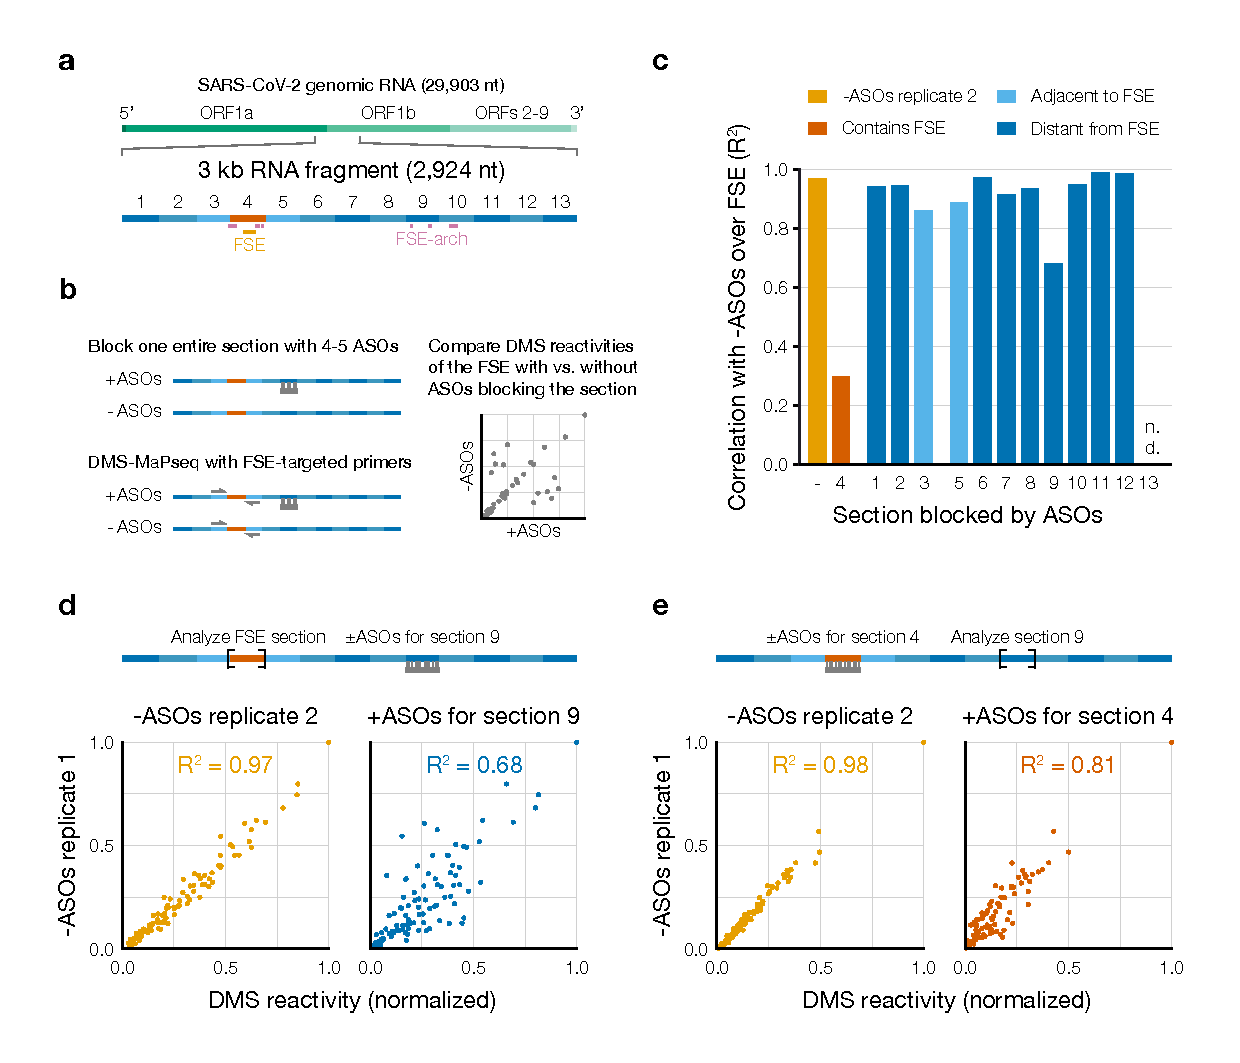
\includegraphics[height=0.95\textheight]{../MainFigures/fig2.pdf}
	\caption{}
	\label{rrna}
\end{figure}


\subsection{SARS-CoV-2 tiling}

Aside from ribosomes, many of the best-characterized, functional long-range RNA--RNA interactions occur in the genomes of RNA viruses~\cite{Nicholson2014}.
Coronaviruses regulate translation of their first open reading frame (ORF1) using programmed ribosomal frameshifting~\cite{Plant2008}.
In the middle of ORF1, a switch called a frameshift stimulation element (FSE) makes a fraction of ribosomes slip backwards into the -1 reading frame.
Ribosomes that maintain reading frame terminate at a stop codon shortly after the FSE, while those that frameshift bypass that stop codon and reach the end of ORF1.
Why coronaviruses need a frameshifting mechanism remains an open question~\cite{Allan2023}, yet they all have FSEs~\cite{Plant2008}.

Every coronaviral FSE contains a ``slippery site" (UUUAAAC) and a structure characterized as a pseudoknot in multiple species~\cite{Brierley1989,Herald1993,Plant2005b}.
Indeed, the isolated core of the SARS coronavirus 2 (SARS-CoV-2) FSE was shown to fold into a pseudoknot with three stems~\cite{KZhang2021,Jones2022}.
However, we discovered that when FSE is in its natural place in the SARS-CoV-2 genome, pseudoknot stem 1 is disassembled while an alternative stem 1 folds~\cite{Lan2022}.
Others identified a long-range RNA--RNA interaction encompassing the FSE, a structure they named the ``FSE-arch"~\cite{Ziv2020}.
These findings hinted that the pseudoknot is not the only coronaviral RNA structure involved in frameshifting.

We applied SEARCH-MaP to determine the ensemble of structures into which the SARS-CoV-2 FSE folds.
To a 2,924 nt segment of the SARS-CoV-2 genome centered on the putative FSE-arch~\cite{Ziv2020}, we added (separately) thirteen groups of DNA ASOs (Figure \ref{tiles}a).
Each group contained four or five ASOs targeting a contiguous 213-244 nt section of the RNA.
After adding each group of ASOs, we performed DMS-MaPseq with two pairs of RT-PCR primers: flanking the ASO target site (to confirm binding) and flanking the 5' FSE-arch (to detect structural changes).
Every ASO group bound properly, evidenced by a decrease in DMS reactivities over its target site (SFIG).

\begin{figure}[H]
	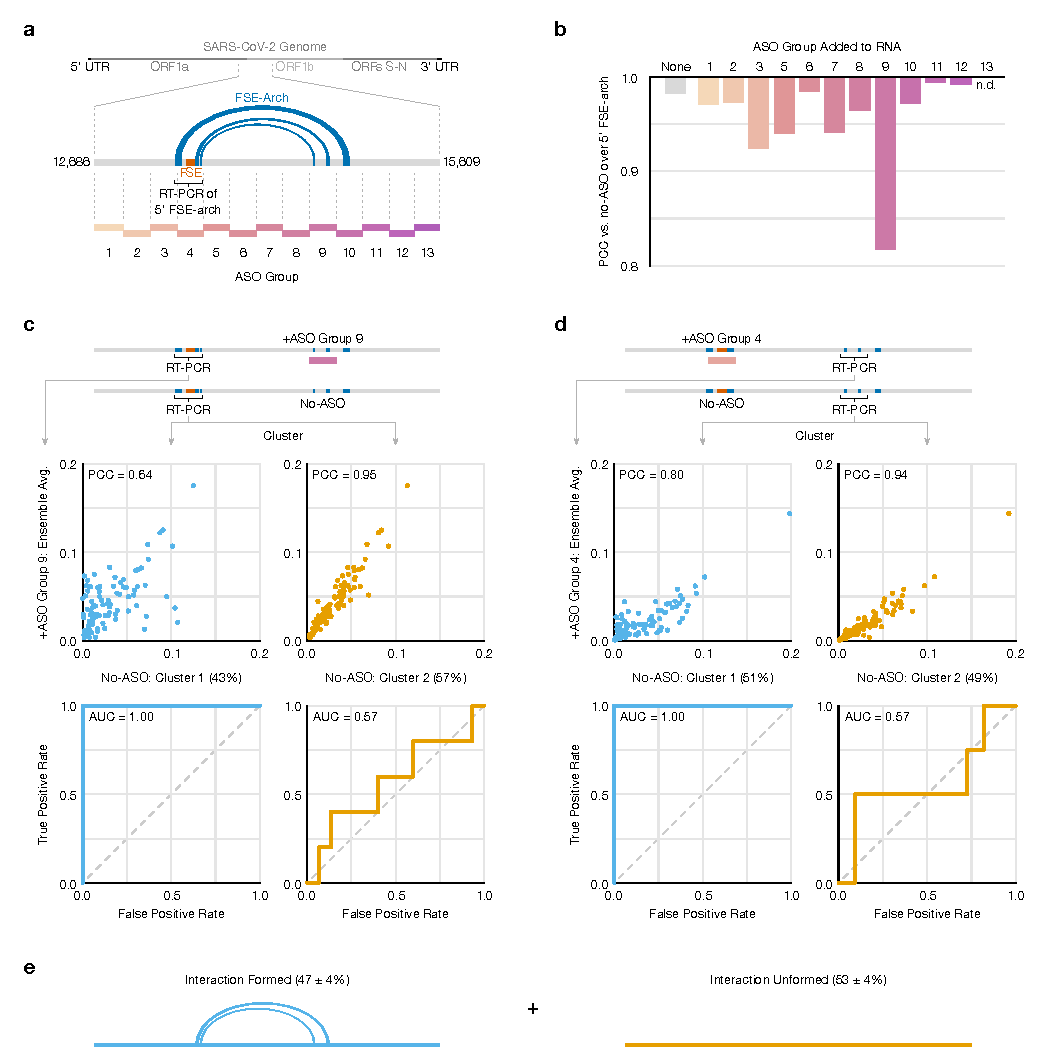
\includegraphics[width=\textwidth]{../MainFigures/sars2-tile/sars2-tile.pdf}
	\caption{\textbf{Characterization of a long-range RNA--RNA interaction in SARS-CoV-2.} \textbf{(a)}~The 2,924 nt segment of the SARS-CoV-2 genome containing the frameshift stimulation element (FSE) and putative FSE-arch~\cite{Ziv2020}. The target of each ASO group is indicated by dotted lines; lengths are to scale. \textbf{(b)}~Pearson correlation coefficient (PCC) of the DMS reactivities over the 5' FSE-arch between each sample and one no-ASO control; n.d. = no data. \textbf{(c)}~(Top) Scatter plots of DMS reactivities over the 5' FSE-arch comparing each cluster of the no-ASO sample to the sample with ASO group 9; each point is one position in the 5' FSE-arch. (Bottom) Receiver operating characteristic (ROC) curves comparing each cluster of the no-ASO sample to the two inner stems of the FSE-arch. \textbf{(d)}~Like (c) but over the 3' FSE-arch, and comparing to the sample with ASO group 4. \textbf{(e)}~Model of the inner two stems in the ensemble of structures formed by the 2,924 nt segment.}
	\label{tiles}
\end{figure}

To quantify structural changes over the 5' FSE-arch, we calculated the Pearson correlation coefficient (PCC) of the DMS reactivities after adding each ASO group versus one no-ASO control (Figure \ref{tiles}b).
A replicate no-ASO sample confirmed the DMS reactivities were reproducible (PCC = 0.98).
Among the ASO groups, group 9 perturbed the 5' FSE-arch the most (PCC = 0.82), and by a large margin (0.11), evidencing that the structures it targets -- the two inner stems of the FSE-arch -- exist.
ASO group 10 had no effect on the 5' FSE-arch (PCC = 0.97), suggesting that its target -- the outer stem -- does not exist or is more sensitive to its environment than are the two inner stems.

We next sought to determine in what fraction of molecules the two inner stems of the FSE-arch fold.
Using SEISMIC-RNA, we clustered reads from the 5' side of the FSE-arch for the no-ASO control and found two distinct clusters, with a 43\%/57\% split.
To determine if these clusters corresponded to the two inner stems formed and unformed, we compared their DMS reactivities to those after adding ASO group 9, which blocks the two inner stems (Figure \ref{tiles}c, top).
Cluster 2 had similar DMS reactivities (PCC = 0.95), indicating that it corresponds to the unformed state.
Meanwhile, cluster 1 had distinct DMS reactivities (PCC = 0.64), suggesting that it corresponds to the two inner stems forming.

To further verify this correspondence, we leveraged the preexisting model of the FSE-arch~\cite{Ziv2020}.
If cluster 1 did correspond to the two inner stems formed, then we would expect its DMS reactivities to agree well with their structures (i.e. paired and unpaired bases should have low and high mutation rates, respectively) and those of cluster 2 to agree much less.
We quantified this agreement using receiver operating characteristic (ROC) curves (Figure \ref{tiles}c, bottom).
The area under the curve (AUC) for cluster 1 was 1.0, indicating perfect agreement with the two inner stems of the FSE-arch, while that of cluster 2 (AUC = 0.57) was close to null (0.50).
This result further supports that cluster 1 (43\%) corresponds to the two inner stems formed, and cluster 2 (57\%) to these stems unformed.

If the RNA really exists as an ensemble of the two inner stems formed and unformed, then we would also expect the 3' side of the FSE-arch to cluster into "formed" and "unformed" states.
To investigate, we performed RT-PCR with primers flanking the 3' side of the inner two stems -- both without ASOs and with ASO group 4 (targeting the 5' side of the FSE-arch).
We clustered the no-ASO control and found -- similar to the previous result -- that cluster 1 (51\%) matched the structure of the inner two stems (AUC = 1.0), while cluster 2 (49\%) agreed with the DMS reactivities (PCC = 0.94) after blocking the FSE-arch with ASO group 4 (Figure \ref{tiles}d).
We concluded that the RNA exists as an ensemble of structures in which the two inner stems of the FSE-arch form in 47\% ± 4\% of molecules (Figure \ref{tiles}e).
This result is consistent with our previous suggestion that a stem similar to the FSE-arch constitutes 45\% of the ensemble in cells infected with SARS-CoV-2~\cite{Lan2022}.


\subsection{The frameshifting pseudoknot competes with the long-range interaction}

We refined the model of the long-range interaction using the mutational profiling data from both clusters that corresponded to this interaction forming (Figure \ref{tiles}c, d).
We predicted the structure of a 1,799 nt segment of the genome centered on the long-range interaction using RNAstructure Fold \cite{Mathews2004a}.
The minimum free energy structure (Figure \ref{lnas}) contained not only the two inner stems of the FSE-arch (LS1 and LS2a/b) but also two additional stems that were not part of the original FSE-arch model~\cite{Ziv2020} (LS3a/b and LS4).
The structure also contained the alternative stem 1 (AS1) that we had previously discovered~\cite{Lan2022}, which encircles the attenuator hairpin (AH)~\cite{Su2005}.
Because we had collected DMS-MaPseq data on both ends of LS3a/b, but only the 5' end of LS4, we focused on LS3a/b.

To our surprise, LS2b, LS3a/b, and LS4 of the new model penetrate into structures within the FSE pseudoknot that is widely thought to stimulate frameshifting -- LS2b overlaps with PS2, LS3 with PS3, and LS4 with PS1.
We had previously shown that AS1 also overlaps with and seems to outcompete PS1~\cite{Lan2022}.
If these stems existed, then they would be mutually exclusive with the FSE pseudoknot, which suggests that the long-range interaction could inhibit the formation of the pseudoknot and possibly regulate the rate of frameshifting.

Thus, we verified these structures of the long-range interaction using SEARCH-MaP.
We performed SEARCH-MaP on the same 1,799 nt segment for which we had predicted the structure, this time with shorter LNA/DNA mixmer ASOs (15-20 nt) to reach single-stem precision.
Each ASO targeted a single stem in the downstream portion of the interaction, and we measured the change in DMS reactivities of the FSE.
ASOs targeting the 3' sides of LS1 and LS2a perturbed the DMS reactivities in exactly the expected locations on the 5' sides (Figure \ref{lnas}b).
Binding an ASO to the 3' side of LS2b caused a larger perturbation with more off-target effects, likely because this stem overlaps with stem 2 of the pseudoknot (PS2), so blocking it with an ASO could promote pseudoknot formation.
Blocking LS3b also resulted in a main effect around the intended location, with one off-target effect upstream, suggesting that there may be another RNA--RNA interaction with the pseudoknot and this upstream region.
These results show that stems LS1, LS2a/b, and LS3b in the refined model of the long-range interaction do exist and can be detected with SEARCH-MaP -- cleanly if the stem does not interact with anything else, otherwise with off-target effects.

Assuming that all stems in Figure \ref{lnas}a do exist, we found that there are six possible structure models resulting from all possible combinations of non-overlapping stems (Figure \ref{lnas}c).
We ordered these models from most long-range character (A) to most pseudoknot-like character (F).
We then determined whether each model actually exists in the ensemble and estimated its proportion.

We found that our no-ASO control clustered reproducibly up to 6 clusters (SFIG).
For each cluster, we found how well it agreed with each structure model by calculating the area under the receiver operating characteristic curve (AUC-ROC).
We graph the results as a heatmap with clusters on the x-axis, in order of and their widths indicating their proportions in the ensemble, and the models on the y-axis.
We consider a cluster and model to be consistent with each other if the AUC-ROC is at least 0.90, and explicitly print all such AUC-ROC values.
We found that model C -- in which AS1 folds along with stems PS2 and PS3 of the pseudoknot -- was consistent with three clusters representing 52\% of the ensemble (Figure \ref{lnas}d, top).
Model A -- where the full long-range interaction forms -- was consistent with one cluster (20\%).
No clusters were consistent with the pseudoknot (Model F); the least-abundant cluster (7\%) came close with an AUC-ROC of 0.88.
The remaining cluster (21\%) was not even close to being consistent with any model, suggesting that there are still other structures in the ensemble besides those in Figure \ref{lnas}c.

These results suggested to us that the primary competitors of the pseudoknot are AS1 and LS2b, since both are present in the most abundant model, C (52\%), while LS3 and LS4 fold in model A, which is only 20\% of the ensemble.
We thus reasoned that if the long-range interaction does actually compete with the pseudoknot, then blocking AS1 and LS2b simultaneously should allow the pseudoknot to fold, while blocking either would have a much smaller effect on the pseudoknot.
To test this hypothesis, we repeated the above experiment while adding an ASO targeting either AS1 or just the part of LS2b that overlaps with the pseudoknot, or both ASOs together.
Blocking AS1 (Figure \ref{lnas}d, left) reduced the proportion of clusters consistent with AS1 (Models A, B, and C) from 72\% to 16\%, as expected; it also resulted in two clusters consistent with the pseudoknot (56\% total) and one cluster (20\%) consistent with Model D, which includes PS1.
Blocking the part of LS2b that seems to overlap with PS2 (Figure \ref{lnas}d, right) eliminated Model A but not Model C (as expected, since Model A includes LS2b, while Model C does not), and also produced one cluster (13\%) that was consistent with the pseudoknot.
Blocking both AS1 and LS2b together (Figure \ref{lnas}d, bottom) forced the entire ensemble into the pseudoknot state, with 87\% of the ensemble highly consistent with Model F (AUC-ROC = 0.97) and the remaining 13\% still somewhat consistent (AUC-ROC = 0.87).
Thus, we conclude that the long-range interaction -- particularly LS2b -- along with AS1, does compete with the pseudoknot.

\begin{figure}[ht]
	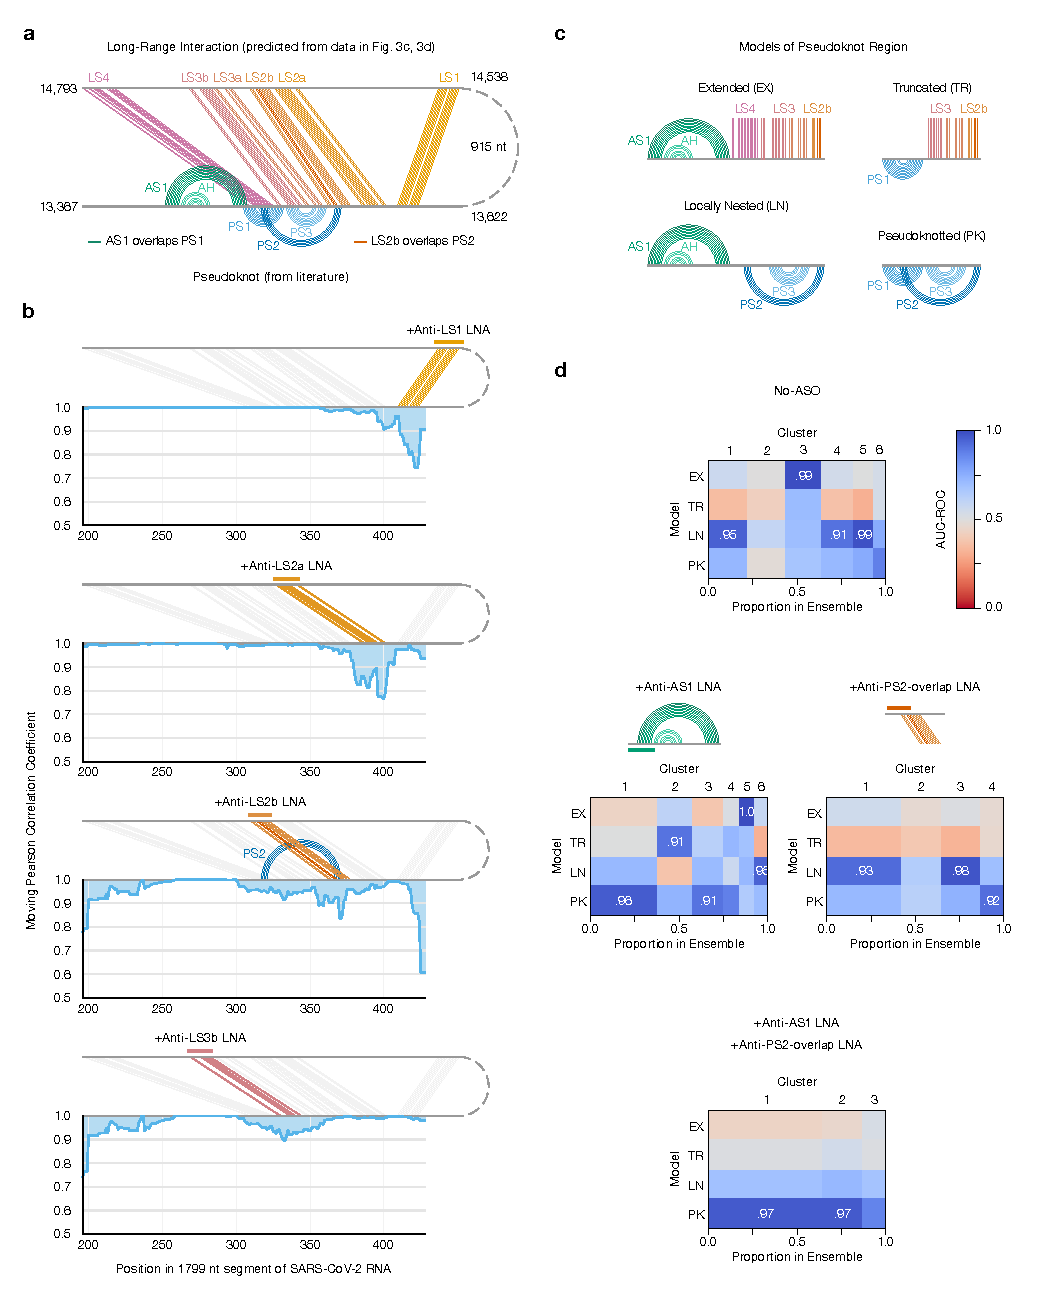
\includegraphics[width=\textwidth]{../MainFigures/lnas/lnas.pdf}
	\caption{}
	\label{lnas}
\end{figure}


\subsection{Frameshift stimulating elements of multiple coronaviruses participate in long-range RNA--RNA interactions}

We hypothesized that similar long-range interactions could exist in other coronaviruses -- particularly other SARS-related viruses.
To test this hypothesis, we performed SEARCH-MaP with FSE-targeted ASOs on 1,799 nt segments from eight selected coronaviruses.


\subsubsection{Computational and experimental screening identifies eight coronaviruses with potential long-range interactions}

As of December 2021, the NCBI Reference Sequence Database~\cite{OLeary2016} contained 62 complete genomes of coronaviruses.
To focus on those likely to have long-range interactions involving the FSE, we predicted the likelihood that each base in a 2,000 nt section surrounding the FSE would pair with a base in the FSE (SFIG).
Based on these predicted interactions, we selected ten coronaviruses -- at least one from each genus (SFIG) -- including SARS-CoV-2 as a positive control.
Within the genus \textit{Betacoronavirus}, we included all three SARS-related viruses -- SARS coronaviruses 1 (\verb|NC_004718.3|) and 2 (\verb|NC_045512.2|) and bat coronavirus BM48-31 (\verb|NC_014470.1|) -- because they clustered into their own structural outgroup.
The other three strains of \textit{Betacoronavirus} that we selected were MERS coronavirus (\verb|NC_019843.3|) with a predicted interaction at positions 510-530; and human coronavirus OC43 (\verb|NC_006213.1|) and murine hepatitis virus strain A59 (\verb|NC_048217.1|), both with a predicted upstream interaction at positions 10-20.
We selected two strains of \textit{Alphacoronavirus}: transmissible gastroenteritis virus (\verb|NC_038861.1|) and bat coronavirus 1A (\verb|NC_010437.1|), predicted to have interactions at positions 440-460 and 350-360, respectively.
Avian infectious bronchitis virus strain Beaudette (\verb|NC_001451.1|) -- a strain of \textit{Gammacoronavirus} -- was predicted to have a strong interaction at positions 330-350, while common moorhen coronavirus HKU21 (\verb|NC_016996.1|) was the species of \textit{Deltacoronavirus} with the most promising FSE interactions.

We reasoned that if an FSE does interact with a distant RNA element, then removing that element by truncating the RNA would break the interaction, causing a structural change in the FSE that could be detected though chemical probing.
For each of the ten coronaviruses that passed the computational screen, we \textit{in vitro} transcribed and performed DMS-MaPseq~\cite{Zubradt2016} on both a 239 nt segment comprising the FSE and minimal flanking sequences and a 1,799 nt segment encompassing the FSE and all sites with which it was predicted to interact.
All coronaviruses except for human coronavirus OC43 and MERS coronavirus showed differences in their DMS reactivity profiles between the 239 nt and 1,799 nt segments (SFIG), suggesting long-range interactions involving the FSE.

\subsubsection{SEARCH-MaP reveals long-range interactions involving the FSE in four other coronaviruses}

To determine which RNA elements the FSE base-pairs with in each coronavirus, we performed SEARCH-MaP on the 1,799 nt RNA segment using DNA ASOs targeting the vicinity of the FSE (Figure \ref{covs}).
The rolling Spearman correlation coefficient (SCC) between the +ASO and no-ASO mutational profiles dipped below 0.9 at the ASO target site in every coronavirus segment, confirming the ASOs bound and altered the structure.

To confirm we could detect long-range interactions, we compared the rolling SCC for the SARS-CoV-2 segment to our model of the long-range interaction (Figure \ref{lnas}a, green).
The SCC dipped below 0.9 at positions 1,483-1,560 and at 1,611-1,642, which coincide with stems LS2a-LS3b (positions 1,476-1,550 within the 1,799 nt segment) and stem LS4 (positions 1,600-1,622) of the long-range interaction.
These dips were the two largest downstream of the FSE; although others (corresponding to no known base pairs) existed, they were barely below 0.9 and could have resulted from base pairing between these regions and other (non-FSE) regions.
Near LS1 (positions 1,367-1,381), the SCC dipped only slightly to a minimum of 0.95, presumably because LS1 is the smallest (15 nt) and most isolated long-range stem.
Therefore, this method was sensitive enough to detect all but the smallest long-range stem, and specific enough that the two largest dips corresponded to validated base pairs.

We found similar long-range interactions in SARS-CoV-1 and another SARS-related virus, Bat coronavirus BM48-31.
Both viruses showed dips in SCC at roughly the same positions as LS2a-LS4 in SARS-CoV-2, indicating that they have homologous structures.
SARS-CoV-1 also had a wide dip below 0.9 at positions 1,284-1,394, corresponding to a homologous LS1.
Thus, three SARS-related viruses share this multi-stemmed long-range interaction involving the FSE, suggesting this structure is functional.

In every other species except common moorhen coronavirus, we found prominent dips in SCC at least 200 nt from the ASO target site.
To model potential base pairing between these dip positions and the FSE, we used the Fold program from RNAstructure~\cite{Mathews2004a} with the no-ASO ensemble average mutational profiles as DMS constraints~\cite{Cordero2012}.
Predictions based on ensemble averages (of all structural states) generally underperform those based on clustered mutational profiles (of fewer states or one state); the ensemble average prediction for SARS-CoV-2 included LS1 and LS2b but missed the other long-range stems.
Nevertheless, we found long-range base pairs consistent with the SEARCH-MaP data for both murine hepatitis virus and transmissible gastroenteritis virus (Figure \ref{covs}, orange).
We conclude that long-range interactions involving the FSE occur more widely than in just SARS-CoV-2, including in \textit{Alphacoronavirus} species.


\begin{figure}[ht]
	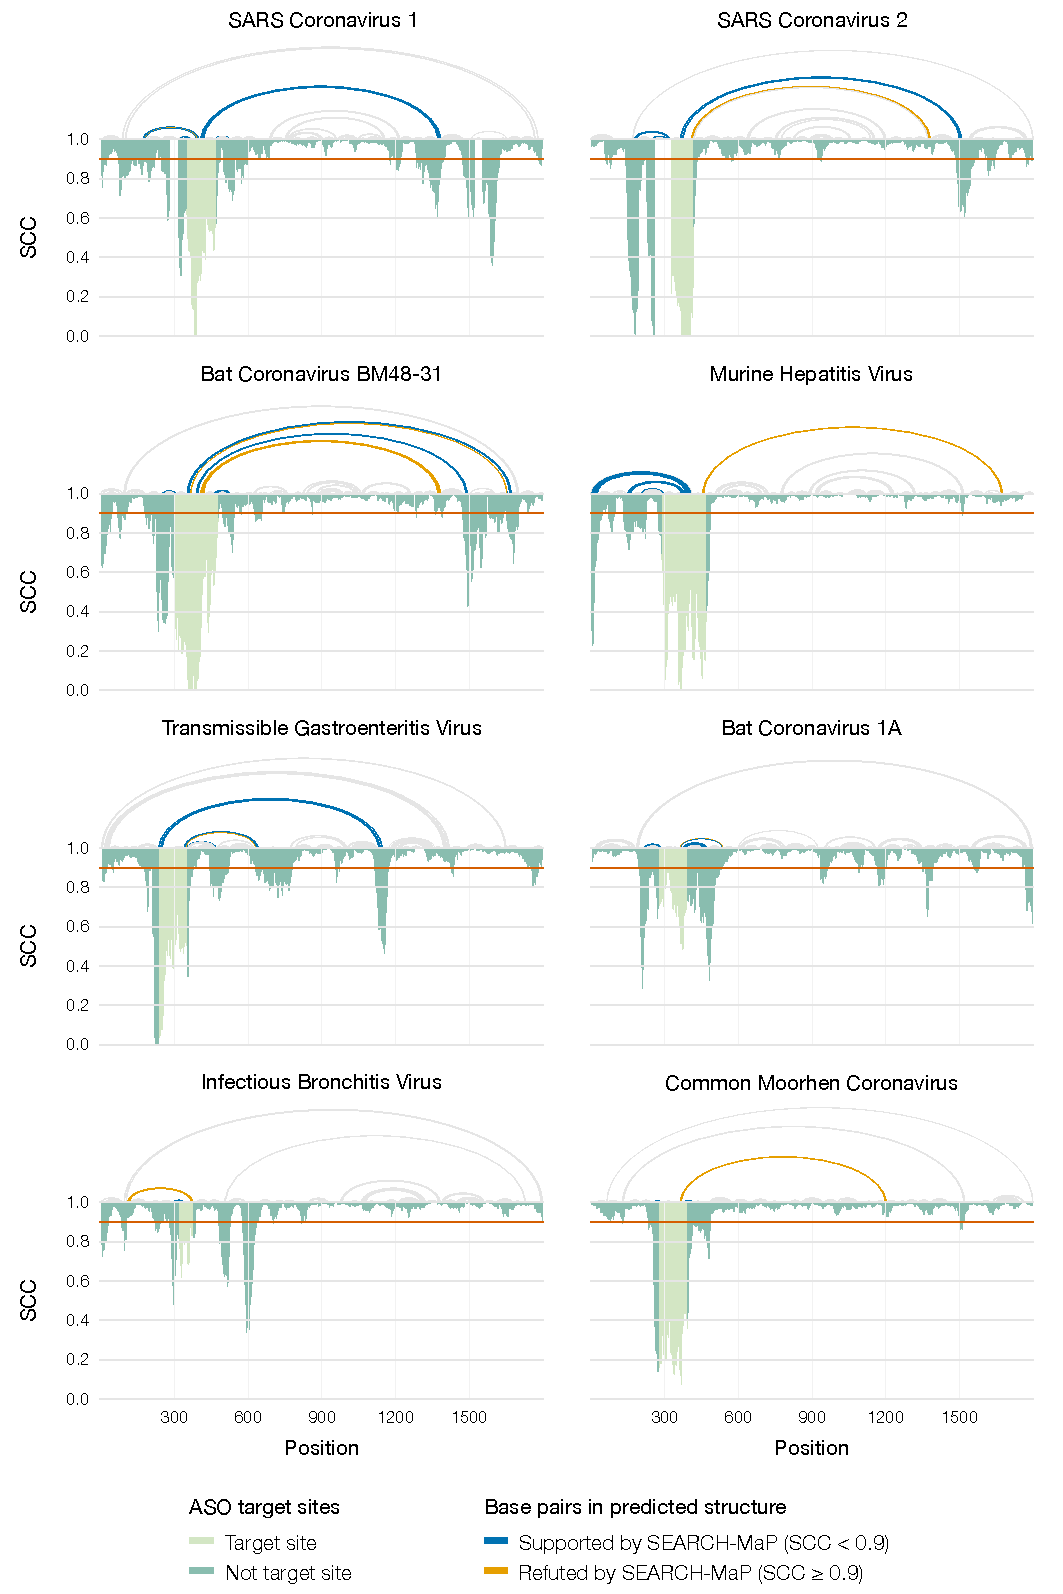
\includegraphics[height=0.95\textheight]{../MainFigures/covs/covs.pdf}
	\caption{}
	\label{covs}
\end{figure}


\subsection{}

We 
To verify that the long-range interaction also forms in live transmissible gastroenteritis virus (TGEV), we treated TGEV-infected ST cells with DMS (two biological replicates) and performed DMS-MaPseq (two technical replicates per biological replicate).
The DMS reactivities were highly reproducible over the whole TGEV genome (\textit{r} = 0.96-0.97, SFIG).
As expected, they differed from those of the 1.8 kb segment \textit{in vitro} (\textit{r} = 0.82, SFIG), showing why it is necessary to verify the long-range interaction in TGEV-infected cells.

First, to determine whether the FSE and the region with which it may interact form alternative structures, we amplified and deeply sequenced these two regions from each sample.
Clustering the reads using SEISMIC-RNA revealed that both regions adopt at least two alternative structures.
The two clusters of the downstream region differed most around positions 1,120-1,140 -- the site of the 3' end of the predicted long-range interaction.
In cluster 1 (63\% of the ensemble), bases 1,129-1,136 (all part of the predicted interaction) had DMS reactivities less than 0.01; while in cluster 2, the DMS reactivities were all greater than 0.01.
This result suggests that cluster 1 corresponds to the state in which the long-range interaction forms.



\end{document}
